% Solutions to the exercises of Chapter 9. Numbers: code/solutions/sol09.py
\documentclass[../solutions_manual.tex]{subfiles}
\begin{document}
\ifSubfilesClassLoaded{\setcounter{chapter}{8}}{}% NN-1 when built standalone
\setcounter{chapter}{8}% NN-1, so this chapter is numbered NN
\chapter{Where Preferences Come From}\label{sol09}

All exercises use the formation equation~\eqref{ch09:eq:formation},
\[
\theta_{i,t+1} = \rho\,\theta_{i,t} + (1-\rho)\bar\theta + \mu\Bigl(\sum_jW^I_{ij}r_{j,t} - r^*\Bigr),
\]
with $t$ in generations and $\kappa := \mu/(1-\rho)$ the formation multiplier. With a constant signal $s$ the solution is $\theta_t = \theta^* - (\theta^* - \theta_0)\rho^t$, with $\theta^* = \bar\theta + \kappa(s - r^*)$; this closed form is used repeatedly. Every number is printed by the script \nolinkurl{code/solutions/sol09.py}.

%% ---------------------------------------------------------------------
\exercisesolution{9.1}{The formation equation by hand}

\solpart{a} With $\rho = 0.8$, $\bar\theta = 1$, $\mu = 0.2$, $r = 0.15$ and $r^* = 0.1$, the map is $\theta_{t+1} = 0.8\,\theta_t + 0.2 + 0.2(0.05) = 0.8\,\theta_t + 0.21$. From $\theta_0 = 0.5$, $\theta_1 = 0.8(0.5) + 0.21 = 0.61$, $\theta_2 = 0.8(0.61) + 0.21 = 0.698$, and so on:
\begin{center}
\small
\setlength{\tabcolsep}{3pt}
\begin{tabular}{ccccccccccc}
\toprule
$t$ & 1 & 2 & 3 & 4 & 5 & 6 & 7 & 8 & 9 & 10 \\
\midrule
$\theta_t$ & 0.6100 & 0.6980 & 0.7684 & 0.8247 & 0.8698 & 0.9058 & 0.9347 & 0.9577 & 0.9762 & 0.9909 \\
\bottomrule
\end{tabular}
\end{center}

\solpart{b} $\theta^* = 0.21/(1 - 0.8) = 1.05$, i.e.\ $\bar\theta + \kappa(r - r^*) = 1 + 1(0.05)$ (Proposition~\ref{ch09:prop:steady}, eq.~\eqref{ch09:eq:steady}). The deviation obeys $\theta_{t+1} - \theta^* = 0.8(\theta_t - \theta^*)$, so $\theta_t = 1.05 - 0.55(0.8)^t$, which reproduces the table (check: $1.05 - 0.55(0.8)^{10} = 0.9909$). Since $|0.8| < 1$ the map is a contraction and $\theta_t \to 1.05$ from any $\theta_0$. The return is constant, so there is no feedback and the local rate of Proposition~\ref{ch09:thm:hysteresis} is $\lambda = \rho$.

\solpart{c} Trajectories (both parts; every second generation):
\begin{center}
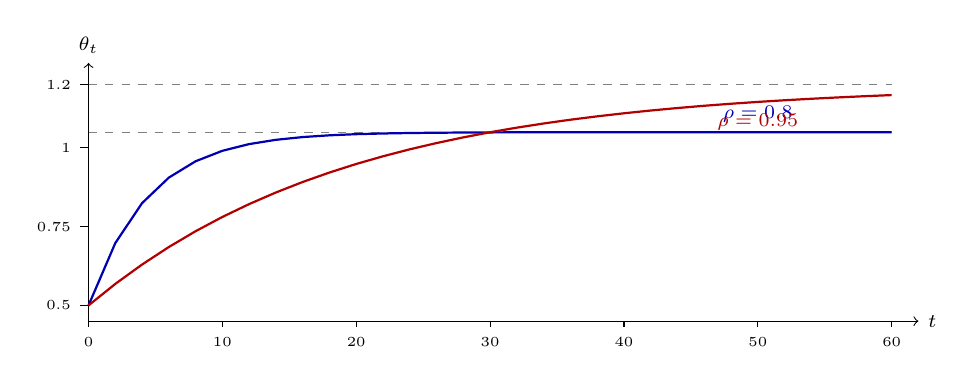
\begin{tikzpicture}[x=0.17cm, y=4cm]
\draw[->] (0,0.45) -- (62,0.45) node[right, font=\scriptsize] {$t$};
\draw[->] (0,0.45) -- (0,1.27) node[above, font=\scriptsize] {$\theta_t$};
\foreach \xx in {0,10,20,30,40,50,60} \draw (\xx,0.45) -- (\xx,0.43) node[below, font=\tiny] {\xx};
\foreach \yy in {0.5,0.75,1,1.2} \draw (0,\yy) -- (-0.6,\yy) node[left, font=\tiny] {\yy};
\draw[dashed, gray] (0,1.05) -- (60,1.05); \draw[dashed, gray] (0,1.2) -- (60,1.2);
\draw[blue!70!black, thick] plot coordinates {(0,0.5000) (2,0.6980) (4,0.8247) (6,0.9058) (8,0.9577) (10,0.9909) (12,1.0122) (14,1.0258) (16,1.0345) (18,1.0401) (20,1.0437) (22,1.0459) (24,1.0474) (26,1.0483) (28,1.0489) (30,1.0493) (32,1.0496) (34,1.0497) (36,1.0498) (38,1.0499) (40,1.0499) (42,1.0500) (44,1.0500) (46,1.0500) (48,1.0500) (50,1.0500) (52,1.0500) (54,1.0500) (56,1.0500) (58,1.0500) (60,1.0500)};
\draw[red!70!black, thick] plot coordinates {(0,0.5000) (2,0.5683) (4,0.6298) (6,0.6854) (8,0.7356) (10,0.7809) (12,0.8217) (14,0.8586) (16,0.8919) (18,0.9219) (20,0.9491) (22,0.9735) (24,0.9956) (26,1.0155) (28,1.0335) (30,1.0498) (32,1.0644) (34,1.0776) (36,1.0896) (38,1.1003) (40,1.1100) (42,1.1188) (44,1.1267) (46,1.1339) (48,1.1403) (50,1.1461) (52,1.1514) (54,1.1561) (56,1.1604) (58,1.1643) (60,1.1678)};
\node[blue!70!black, font=\scriptsize, above] at (50,1.05) {$\rho = 0.8$};
\node[red!70!black, font=\scriptsize, below] at (50,1.14) {$\rho = 0.95$};
\end{tikzpicture}
\end{center}
``90\% of the steady state'' has two readings; state which one you use.
\begin{itemize}
\item \emph{Level:} $\theta_t \ge 0.9\,\theta^* = 0.945$ requires $0.55(0.8)^t \le 0.105$, i.e.\ $t \ge 7.42$. It is first reached at $t = 8$ ($\theta_8 = 0.9577$).
\item \emph{Gap:} 90\% of the initial gap closed requires $0.8^t \le 0.1$, i.e.\ $t \ge 10.32$, first reached at $t = 11$ ($\theta_{10}$ has closed $89.3\%$).
\end{itemize}
The half-life is $\ln 2/\ln 1.25 = 3.11$ generations (eq.~\eqref{ch09:eq:halflife}).

\solpart{d} With $\rho = 0.95$, $\theta_{t+1} = 0.95\,\theta_t + 0.05 + 0.01 = 0.95\,\theta_t + 0.06$, and $\theta^* = 1.20$. The steady state changes too, because $\kappa = 0.2/0.05 = 4$ instead of $1$. $\theta_1, \ldots, \theta_{10} = 0.535, 0.5682, 0.5998, 0.6298, 0.6584, 0.6854, 0.7112, 0.7356, 0.7588, 0.7809$. The level criterion is met at $t = 35$ (exact $34.38$) and the gap criterion at $t = 45$ (exact $44.89$); the half-life is $13.5$ generations.

Convergence is about $4.3$ times slower, the ratio $\ln 0.8/\ln 0.95$. Raising $\rho$ with $\mu$ fixed changes \emph{two} things: the speed ($1 - \rho$) and the long-run sensitivity ($\kappa$). The slow--fast scaling of Appendix~9B separates them by holding $\kappa$ fixed. \emph{Common mistake:} attributing the whole difference between the two trajectories to persistence; part of it is that the $\rho = 0.95$ dynasty is heading to a higher steady state.

%% ---------------------------------------------------------------------
\exercisesolution{9.2}{Heterogeneous steady states}

Example~\ref{ch09:ex:two_steady}: $\rho = 0.8$, $\mu = 0.3$ ($\kappa = 1.5$), $\bar\theta = 1$, $r^* = 0.1$, $g_M(\theta) = 0.05 + 0.1\theta$ and $g_T(\theta) = 0.03 + 0.02\theta$. With $\mathbf g = \mathbf a + G\btheta$, $\mathbf a = (0.05, 0.03)'$ and $G = \operatorname{diag}(0.1, 0.02)$, case~(b) of Proposition~\ref{ch09:prop:steady} gives the unique steady state
\[
\btheta^* = \Bigl(I - \kappa W^IG\Bigr)^{-1}\Bigl(\bar\theta\ones + \kappa(W^I\mathbf a - r^*\ones)\Bigr).
\]

\solpart{a} With $W^I = I$ the system decouples: $\theta_M = 1 + 1.5(0.05 + 0.1\theta_M - 0.1)$, so $0.85\,\theta_M = 0.925$ and $\theta_M^* = 1.0882$; and $0.97\,\theta_T = 0.895$, so $\theta_T^* = 0.9227$. The gap is $0.1656$. Both maps have slope below one ($0.83$ and $0.806$), so each steady state is unique and globally stable.

\solpart{b} With $W^I = \begin{pmatrix}0.7 & 0.3\\0.3 & 0.7\end{pmatrix}$, the linear system gives $\btheta^* = (1.0332, 0.9709)$. The returns are then $(0.1533, 0.0494)$ and the signals $W^I\mathbf r = (0.1222, 0.0806)$. The gap shrinks to $0.0623$, matching the example. The local rate is $\lambda = \rho(\rho I + \mu W^IG) = 0.822$ (Proposition~\ref{ch09:thm:hysteresis}).

\solpart{c} \emph{The gap vanishes exactly at $w = 0.5$.} Subtract the two steady-state equations with $W^I = \begin{pmatrix}1-w & w\\ w & 1-w\end{pmatrix}$:
\[
\theta_M^* - \theta_T^* = \kappa\bigl[((1-w)r_M + wr_T) - (wr_M + (1-w)r_T)\bigr] = \kappa\,(1 - 2w)\,(r_M^* - r_T^*).
\]
The anchor and the reference cancel; only the difference in \emph{signals} remains. At $w = 0.5$ both rows of $W^I$ are equal, both agents observe the same signal, and since everything else in~\eqref{ch09:eq:steady} is common, $\theta_M^* = \theta_T^*$. Here both equal $1.000$, with returns $(0.15, 0.05)$. Conversely, if the gap is zero then $\theta_M = \theta_T = \theta$ and $r_M - r_T = 0.02 + 0.08\theta > 0$ for $\theta > -0.25$, so $1 - 2w = 0$. The formula, verified numerically:
\begin{center}
\begin{tabular}{lccccc}
\toprule
$w$ & 0.3 & 0.4 & 0.5 & 0.6 & 1.0 \\
\midrule
$\theta_M^* - \theta_T^*$ & $+0.0623$ & $+0.0306$ & $0.0000$ & $-0.0294$ & $-0.1371$ \\
\bottomrule
\end{tabular}
\end{center}
The gap does \emph{not} vanish because returns equalize: they remain $0.15$ vs $0.05$. Beyond $w = 0.5$ it reverses, and each agent is calibrated mostly on the other sector's returns. The answer is not ``as large as possible''.

\solpart{d} Raising $W^I_{12}$ means the Modern agent observes more traditional-sector outcomes; raising $W^I_{21}$, the reverse. Real-world counterparts include school integration and scholarships that put children of both sectors in the same reference groups, mentoring and job networks across sectors, media representation of the other sector's lives, migration links, and, in the other direction, extension workers and public officials embedded in rural communities.

Two cautions from the chapter apply. First, what changes is \emph{information}, not the return functions: a traditional agent calibrated on modern returns may over-aspire relative to what $g_T$ rewards (the Intuition after Proposition~\ref{ch09:thm:self_confirming}). Second, connecting the agents here \emph{lowers} average ambition: the mean steady-state $\theta$ falls from $1.0055$ ($W^I = I$) to $1.0021$ ($w = 0.3$) and $1.000$ ($w = 0.5$). Whether that is good is a welfare question (Chapter~12), not a property of the formation equation.

%% ---------------------------------------------------------------------
\exercisesolution{9.3}{Persistence in female labor supply}

\solpart{a} Substituting $\bar r_t = 0.3\,\theta^F_t$:
\[
\theta^F_{t+1} = 0.85\,\theta^F_t + 0.075 + 0.1(0.3\,\theta^F_t - 0.1) = 0.88\,\theta^F_t + 0.065 .
\]
The steady state is $\theta^{F*} = 0.065/0.12 = 0.5417$. It is unique because the map is affine with slope $0.88 \neq 1$: $\theta = 0.88\theta + 0.065$ has exactly one solution. It is globally stable because $0.88 < 1$. The network effect raises the slope from $\rho = 0.85$ to $\lambda = 0.88$ and slows adjustment (half-life $5.42$ generations instead of $4.27$), as Proposition~\ref{ch09:thm:hysteresis} predicts for $D\mathbf g > 0$.

\solpart{b, c} From $\theta^F_0 = 0.2$ without the war, $\theta^F_t = 0.5417 - 0.3417(0.88)^t$: $\theta^F_{10} = 0.4465$, $\theta^F_{20} = 0.5152$ and $\theta^F_{50} = 0.5411$. With the war, $\theta^F_{10}$ jumps to $0.6$ and the post-war path is $\theta^F_t = 0.5417 + 0.0583(0.88)^{t-10}$: $0.5930$ at $t = 11$, $0.5579$ at $t = 20$, $0.5462$ at $t = 30$ and $0.5420$ at $t = 50$.
\begin{center}
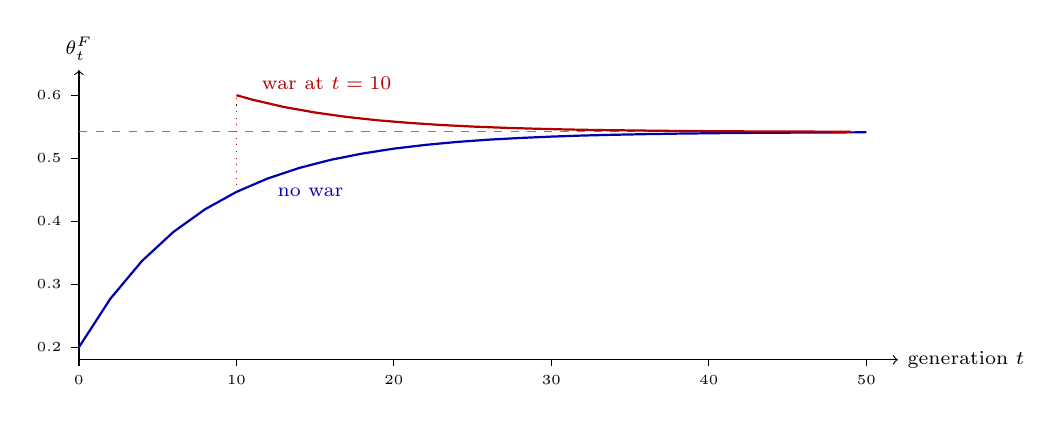
\begin{tikzpicture}[x=0.2cm, y=8cm]
\draw[->] (0,0.18) -- (52,0.18) node[right, font=\scriptsize] {generation $t$};
\draw[->] (0,0.18) -- (0,0.64) node[above, font=\scriptsize] {$\theta^F_t$};
\foreach \xx in {0,10,20,30,40,50} \draw (\xx,0.18) -- (\xx,0.17) node[below, font=\tiny] {\xx};
\foreach \yy in {0.2,0.3,0.4,0.5,0.6} \draw (0,\yy) -- (-0.5,\yy) node[left, font=\tiny] {\yy};
\draw[dashed, gray] (0,0.5417) -- (50,0.5417);
\draw[blue!70!black, thick] plot coordinates {(0,0.2000) (2,0.2771) (4,0.3368) (6,0.3830) (8,0.4188) (10,0.4465) (12,0.4680) (14,0.4846) (16,0.4975) (18,0.5074) (20,0.5152) (22,0.5211) (24,0.5258) (26,0.5294) (28,0.5321) (30,0.5343) (32,0.5360) (34,0.5372) (36,0.5382) (38,0.5390) (40,0.5396) (42,0.5401) (44,0.5404) (46,0.5407) (48,0.5409) (50,0.5411)};
\draw[red!70!black, thick] plot coordinates {(10,0.6000) (11,0.5930) (13,0.5814) (15,0.5725) (17,0.5655) (19,0.5601) (21,0.5560) (23,0.5527) (25,0.5502) (27,0.5483) (29,0.5468) (31,0.5456) (33,0.5447) (35,0.5441) (37,0.5435) (39,0.5431) (41,0.5428) (43,0.5425) (45,0.5423) (47,0.5422) (49,0.5421)};
\draw[red!70!black, dotted] (10,0.4465) -- (10,0.6);
\node[red!70!black, font=\scriptsize, above right] at (11,0.593) {war at $t = 10$};
\node[blue!70!black, font=\scriptsize, below right] at (12,0.468) {no war};
\end{tikzpicture}
\end{center}
$\theta^F$ does \emph{not} return to the pre-war level $0.4465$. The post-war minimum is $0.542$, above it. But the pre-war level was not a steady state: the economy was already converging to $0.5417$. The right comparison is with the no-war path.

\solpart{d} \emph{No permanent effect.} Let $e_t = \theta^{F,\text{war}}_t - \theta^{F,\text{no war}}_t$. Both paths obey the same affine map from $t = 10$ on, so $e_{t+1} = 0.88\,e_t$ and $e_t = (0.6 - 0.4465)(0.88)^{t-10} = 0.1535(0.88)^{t-10} \to 0$. The difference is $0.0810$ at $t = 15$, $0.0428$ at $t = 20$, $0.0119$ at $t = 30$ and $0.0009$ at $t = 50$. Any temporary shock is eventually forgotten, at rate $0.88$ per generation, because the map has a unique, globally stable fixed point.

\emph{What would make it permanent.} Hysteresis needs at least two stable steady states, with the shock moving $\theta$ across the boundary of their basins. That requires the composite map to cross the $45^\circ$ line three times, with slope above one somewhere. An S-shaped return function does this: low returns at low participation (no networks, no childcare, hostile norms), steep returns in a middle range, saturation at high participation (Chapter~10, Example~\ref{ch10:ex:trap}). A large enough wartime jump past the unstable middle steady state would then move society to the high-participation steady state for good. A smaller one would be reversed. In this linear model, $0.88 < 1$ everywhere rules this out.

\emph{Evidence.} \citet{fernandez2004mothers} use cross-state variation in the WWII mobilization rate of men as a shock to the share of men raised by working mothers. They find that wives of such men are more likely to work, a channel of intergenerational preference formation. This fits a model in which a temporary shock persists through $\theta$ for at least a generation. The historical evidence on the war's \emph{direct} effect is more mixed. Goldin (1991, \textit{AER}) argues that the war's direct effect on women's employment was modest, since many wartime entrants had left the labor force by 1950; Acemoglu, Autor and Lyle (2004, \textit{JPE}) find higher female labor supply in 1950 in high-mobilization states. A careful answer distinguishes the short-run reversal (consistent with the linear model) from a longer-run effect transmitted through sons' preferences. The latter is persistence through $\rho$, and it is not by itself evidence of multiple steady states. \emph{Common mistake:} treating any long-lasting effect as hysteresis. With $\rho$ close to one, a single steady state can produce effects that last a century (Example~\ref{ch09:ex:hysteresis}).

%% ---------------------------------------------------------------------
\exercisesolution{9.4}{Aspiration and the smartphone}

\emph{Set-up.} The sectors sit at the steady states of Example~\ref{ch09:ex:two_steady}: $\theta_M^* = 1.0882$, $\theta_T^* = 0.9227$, with returns $r_M = 0.15882$ and $r_T = 0.04845$. The agent is one of many in her sector, so her own $\theta$ does not move the sector returns she observes (the individual case). Before $t = 5$ her signal is $r_T$; from $t = 5$ on it is $0.7\,r_T + 0.3\,r_M$.

\solpart{a} \emph{Old steady state:} $\theta^{\text{old}} = 1 + 1.5(0.04845 - 0.1) = 0.9227$, the sector's value. \emph{New steady state:} $\theta^{\text{new}} = 1 + 1.5(0.7(0.04845) + 0.3(0.15882) - 0.1) = 0.9724$, a gain of $0.0497$. Since $\theta_s^* - \bar\theta = \kappa(r_s - r^*)$ in each sector, the gain is exactly $w\kappa(r_M - r_T) = w(\theta_M^* - \theta_T^*)$. In the long run, the phone closes the share $w = 0.3$ of the Modern--Traditional aspiration gap.

\solpart{b} From $\theta_0 = 0.8$ she first converges toward $0.9227$ ($\theta_5 = 0.8825$). After the phone, $\theta_t = 0.9724 - 0.0899(0.8)^{t-5}$:
\begin{center}
\begin{tabular}{lccccccccc}
\toprule
$t$ & 4 & 5 & 6 & 7 & 8 & 9 & 10 & 11 & 12 \\
\midrule
$\theta_t$ & 0.8724 & 0.8825 & 0.9005 & 0.9148 & 0.9263 & 0.9355 & 0.9429 & 0.9488 & 0.9535 \\
\bottomrule
\end{tabular}
\end{center}
Half of the gap to the new steady state ($0.0899$ at $t = 5$) closes in $\ln 2/\ln(1/0.8) = 3.11$ generations, so it has closed by $t = 9$, four generations ($\approx 100$ years) after the phone. The individual's rate is $\rho = 0.8$, because her own aspiration does not feed back into the returns she observes. If ``the aspiration gap'' means the gap to the Modern sector, half of it is \emph{never} closed at $w = 0.3$; that would take $w = 0.5$.

\solpart{c} \emph{No: it is close to, but not exactly, 100 times}, for two opposite reasons.
\begin{enumerate}
\item \emph{Spillover through the sector's return (a social multiplier).} If the sector's return depends on the sector's average aspiration, $r_T = 0.03 + 0.02\,\bar\theta_T$, then treated agents raise $\bar\theta_T$. That raises $r_T$, which raises everyone's signal, treated or not. Solving the linear system for a treated share $s$, the aggregate effect per treated agent is $1.031$ times the individual effect for small $s$, $1.026$ at $s = 0.5$, and $1.0215 = 1/(1 - \kappa(0.7)(0.02))$ when the whole sector is treated. With 100 phones in a large sector, the total is about $103$ individual effects. The feedback also slows adjustment slightly ($\lambda = 0.804$ instead of $0.8$).
\item \emph{General equilibrium in the observed returns.} If many traditional agents aim at modern-sector outcomes, the modern returns \emph{they} can attain may fall: entry, crowding, credential inflation. As an illustration, suppose the observed modern return falls by $0.05s$. The aggregate effect per treated agent is then $0.983$, $0.794$ and $0.559$ times the individual effect at $s = 0.1$, $0.5$ and $1$.
\end{enumerate}
The individual effect is a partial-equilibrium object, and scaling it up assumes that the return functions do not move. That assumption is what the hint questions, and it is the same caveat as for $\Psi$ (Remark~\ref{ch09:rem:psi}): the answer depends on the perturbation's scale.

%% ---------------------------------------------------------------------
\exercisesolution{9.5}{\citet{bernard2014future} as a $W^I$ perturbation}

\solpart{a} Add a node $f$ (the film's successful farmer, with return $r_{\text{film}}$). For each treated farmer $i \in \mathcal T$, the documentary moves weight $w \in (0,1)$ to $f$ and scales the rest of the row down proportionally:
\[
\Delta W^I_{i\cdot} = w\bigl(\mathbf e_f - W^I_{i\cdot}\bigr)' \quad (i \in \mathcal T), \qquad \Delta W^I_{i\cdot} = 0 \quad (i \notin \mathcal T).
\]
Each row of $\Delta W^I$ sums to zero, so $W^I + \Delta W^I$ stays row-stochastic, and nonnegativity holds for $w \le 1$. The film subject's own row can be anything, since nobody's dynamics depend on $\theta_f$; take $W^I_{f\cdot} = \mathbf e_f'$. This states the perturbation as Definition~\ref{ch09:def:psi} requires: layer $W^I$, rows of the treated, compensation by proportional scaling.

\solpart{b} For a treated farmer whose own return does not respond to her own $\theta$ (the individual case of Exercise~9.4), the signal changes by $w(r_{\text{film}} - \bar r_i)$, where $\bar r_i = \sum_jW^I_{ij}r_j$ is her old signal. Then, by~\eqref{ch09:eq:steady},
\[
\Delta\theta_i^* = \frac{\mu}{1-\rho}\,w\,\bigl(r_{\text{film}} - \bar r_i\bigr).
\]
If her own return responds ($r_i = g_i(\theta_i)$, $g_i' > 0$, $W^I_{ii} > 0$), subtracting the old and new steady-state equations gives
\[
\Delta\theta_i^* = \frac{\kappa\,w\,(r_{\text{film}} - \bar r_i)}{1 - \kappa(1-w)W^I_{ii}\,g_i'}, \qquad \kappa = \frac{\mu}{1-\rho},
\]
and in general $\Delta\btheta^* = (I - \kappa(W^I + \Delta W^I)G)^{-1}\kappa\,\Delta W^I\mathbf r^0$ for affine $\mathbf g$ (case~(b) of Proposition~\ref{ch09:prop:steady}). The effect is proportional to the formation multiplier $\kappa$, the weight $w$ of the new edge, and the \emph{gap} between the film's return and what she observed before. A film about a farmer like her has no effect. The path to $\Delta\theta_i^*$ is $\Delta\theta_{i,T} = \Delta\theta_i^*(1 - \lambda^T)$, with $\lambda = \rho$ in the individual case.

\solpart{c} \emph{Implied $\mu$.} If the six-month effect is read as the impact effect of one period of the formation equation, $\Delta\theta_{i,1} = \mu\,w\,(r_{\text{film}} - \bar r_i)$. A $0.1$ SD effect \illustrative\ then implies
\[
\mu = \frac{0.1\,\sigma_\theta}{w\,(r_{\text{film}} - \bar r_i)} .
\]
For example, $\mu = 1.0$ if $w = 0.1$ and the return gap is $1$ SD of $\theta$; $\mu = 2.0$ if $w = 0.05$; $\mu = 0.5$ if $w = 0.1$ and the gap is $2$ SD. The number is only as good as the assumed $w$ and gap, neither of which the experiment measures.

\emph{The time-scale problem.} The formation equation is per \emph{generation} (about 25 years), and six months is $1/50$ of a generation. Let the six-month process have parameters $(\rho_{6}, \mu_{6})$. Fifty sub-periods with a constant signal aggregate to one generation with
\[
\rho_{\text{gen}} = \rho_6^{50}, \qquad \mu_{\text{gen}} = \mu_6\,\frac{1 - \rho_6^{50}}{1 - \rho_6}, \qquad \frac{\mu_{\text{gen}}}{1 - \rho_{\text{gen}}} = \frac{\mu_6}{1 - \rho_6}.
\]
The ratio $\mu_{\text{gen}}/\mu_6$ is $50$ if $\rho_6 = 1$ (no decay), $39.5$ if $\rho_6 = 0.99$, $18.5$ if $\rho_6 = 0.95$, and $9.95$ if $\rho_6 = 0.9$. A six-month impact identifies $\mu_6$ at best. Mapping it to $\mu_{\text{gen}}$ requires the decay rate $\rho_6$, which one follow-up round cannot reveal. Only the long-run multiplier $\kappa$ is invariant to the period length, and it requires the long-run effect, not the impact. There are further problems:
\begin{itemize}
\item a six-month change may be a revision of \emph{beliefs} (the fast DeGroot channel of Chapter~8), not of preferences (Section~\ref{ch09:sec:beliefs});
\item survey measures of aspirations may respond to experimenter demand;
\item SD units depend on the sample's dispersion, not on the model's $\theta$.
\end{itemize}
\emph{Common mistake:} plugging the six-month coefficient directly into a per-generation $\mu$, which can be off by a factor between $1$ and $50$.

\solpart{d} Yes, if savings respond more than proportionally to $\theta$. Let $s = f(\theta)$ with $f$ convex and $f(0) \le 0$ (no saving without aspiration). By convexity, the tangent at $\theta > 0$ lies below $f$ at $0$: $f(0) \ge f(\theta) - \theta f'(\theta)$. Hence $\theta f'(\theta) \ge f(\theta) - f(0) \ge f(\theta)$, i.e.\ the elasticity $\theta f'(\theta)/f(\theta) \ge 1$. A given percentage change in $\theta$ then produces at least the same percentage change in savings. A $10\%$ rise in $\theta$ raises $s = \theta^2$ by $21.0\%$ and $s = e^\theta - 1$ (at $\theta = 1$) by $16.6\%$, against $10\%$ for a linear $f$. Convexity is natural with a fixed cost of saving or investing: an account, a minimum lumpy investment, or a threshold aspiration above which forward-looking plans begin.

Two caveats. First, in standardized (SD) units the comparison also depends on the dispersion of $s$ relative to $\theta$, so ``larger'' must be stated in comparable units. Second, savings also respond to the information in the film directly, through beliefs about returns, which is not formation. Distinguishing the two needs a design in the spirit of \citet{bursztyn2014understanding}.

%% ---------------------------------------------------------------------
\exercisesolution{9.6}{The $\Psi$ ratio for education}

The outcome is $x = \theta w/p$; the perturbation is a permanent $10\%$ cut in $p$; the horizon is $T = 1$ (Definition~\ref{ch09:def:psi}). Write $x_0 = \theta_0w/p_0$.

\solpart{a} \emph{Enforcement} (fixed $\theta$): $E = \theta_0w/(0.9p_0) - x_0$, so $E/x_0 = 1/0.9 - 1 = 0.1111$, i.e.\ $+11.1\%$. (The first-order approximation $-d\ln p = 10\%$ understates it, because demand is unit-elastic in $p$.)

\solpart{b} \emph{Formation} (new $\theta$ at the new price): $F = 1.05\,\theta_0w/(0.9p_0) - \theta_0w/(0.9p_0)$, so $F/x_0 = 0.05/0.9 = 0.0556$, i.e.\ $+5.6\%$ of the original quantity. The total change is $(E + F)/x_0 = 1.05/0.9 - 1 = 0.1667$, which confirms the decomposition $E_i + F_i = y_i(\btheta_T, W + \Delta W) - y_i(\btheta^0, W)$.

\solpart{c} $\Psi = F/E = 0.0556/0.1111 = 0.500$. The enforcement effect is twice as large. An evaluation that ignores formation captures $1/(1+\Psi) = 2/3$ of the effect at $T = 1$ and misses one third (Remark~\ref{ch09:rem:psi}, item 4).

\solpart{d} With a price cut of fraction $c$ and a preference change of fraction $g$ by horizon $T$,
\[
\frac{E}{x_0} = \frac{c}{1-c}, \qquad \frac{F}{x_0} = \frac{g}{1-c}, \qquad \Psi = \frac{g}{c} .
\]
Hence $\Psi > 1$ iff the induced proportional change in preferences exceeds the proportional price cut, $g > c$. The common factor $1/(1-c)$ cancels because $x$ is multiplicative in $\theta$ and $1/p$. Inside the formation model $g$ is not free. If the economy starts at a steady state and the policy shifts the observed signal by $\Delta s$, then $g(T) = \frac{\kappa\Delta s}{\theta_0}(1 - \lambda^T)$. So $\Psi > 1$ requires:
\begin{enumerate}
\item a large formation multiplier $\kappa = \mu/(1-\rho)$;
\item a policy that changes what the reference group visibly earns (a large $\Delta s$, e.g.\ returns to educated women that girls can observe);
\item a long enough horizon relative to the adjustment rate $\lambda$;
\item a small direct price effect.
\end{enumerate}
\emph{Illustration.} If the $5\%$ at $T = 1$ is the first generation of an adjustment with $\lambda = 0.8$, the long-run change is $g_\infty = 0.05/0.2 = 0.25$, and $\Psi$ rises with the horizon: $0.90$ at $T = 2$, $1.22$ at $T = 3$, $1.68$ at $T = 5$, $2.23$ at $T = 10$, and $2.5$ in the long run. $\Psi > 1$ from $T > 2.29$ generations. The same policy is ``mostly enforcement'' at one generation and ``mostly formation'' at three: $\Psi$ is a property of the perturbation, the outcome and the horizon, not of the economy (Remark~\ref{ch09:rem:psi}).

%% ---------------------------------------------------------------------
\exercisesolution{9.7}{Furtado's demonstration effect}

\solpart{a} The elite's $W^I$ row places $0.4$ on the Center and $0.6$ on the Periphery: travel, media and education abroad give Center consumption a weight comparable to the elite's own society. The row sums to one.

\solpart{b} The observed ``returns'' are the consumption ratios $0.85$ (Center) and $0.70$ (Periphery), so the signal is $0.4(0.85) + 0.6(0.70) = 0.76$. With $\bar\theta = r^* = 0.70$, $\rho = 0.9$ and $\mu = 0.4$ ($\kappa = 4$),
\[
\theta^* = 0.70 + 4\,(0.76 - 0.70) = 0.94 .
\]
The elite consumes $94\%$ of its income, against the sustainable $70\%$. The map has slope $\rho = 0.9$ (the observed ratios do not depend on $\theta$), so the steady state is unique and stable, with half-life $6.6$ generations. Starting from $0.70$, $\theta_t$ is $0.724$, $0.798$, $0.856$, $0.911$ and $0.940$ at $t = 1, 5, 10, 20, 60$.

\solpart{c} With weight $w$ on the Center, $\theta^*(w) = 0.70 + 4w(0.85 - 0.70) = 0.70 + 0.6w$. It exceeds $1$ iff $w > 0.5$: once the Center carries more weight than the elite's own society, the steady state is chronic dissaving. The multiplier $\kappa = 4$ amplifies a modest consumption gap ($0.15$) into a large preference deviation. The model is linear and $\theta > 1$ is outside its meaningful range (Definition~\ref{ch09:def:formation}); read the threshold as the point where the local approximation predicts unsustainable consumption, i.e.\ debt, rents or capital inflows.

\emph{Variant.} If the ``Periphery'' signal were the elite's \emph{own} consumption ratio rather than a fixed $0.70$, the map would have slope $\rho + 0.6\mu = 1.14 > 1$. Its fixed point ($0.529$) would then be unstable, and consumption would run away from it: a self-reinforcing emulation race.

\solpart{d} Each structural lever corresponds to a term of the steady-state formula $\theta^* = \bar\theta + \kappa(w\,c_C + (1-w)c_P - r^*)$:
\begin{itemize}
\item \emph{Lower $w$}: reduce the weight of Center consumption in the elite's reference set, for instance through domestic media and cultural production, or taxes on imported luxury consumption that make Center patterns less visible and less attainable.
\item \emph{Lower $c_C - c_P$ in what is observed}: make the Periphery's own consumption the relevant comparison, which is Furtado's argument for an autonomous cultural project.
\item \emph{Change the anchor or reference} through institutions that stabilize saving norms: pension systems, development banks, savings mandates.
\item \emph{Address the distributional root.} For Furtado, income concentration is what lets a minority emulate the Center. Redistribution shrinks the group whose $W^I$ is Center-oriented, and raises the attainable consumption of the majority, so the observed returns become attainable.
\end{itemize}
The formation equation alone cannot say whether a cross-border edge helps or harms. Here it harms because the returns it carries are not attainable at peripheral incomes (the Prebisch box of Section~\ref{ch09:sec:trap}). \emph{Common mistake:} prescribing ``less information'' as such. The problem is the mismatch between observed and attainable returns, and the book's remedies act on that mismatch: access, income, and what the edge carries.

\end{document}
